 
%\documentclass[aps,prl,a4paper,superscriptaddress,amsmath,amssymb]{revtex4} 
%\usepackage{graphicx,epsfig}
%\usepackage[usenames]{color}



\documentclass[aps,prl,a4paper,superscriptaddress,amsmath,amssymb]{revtex4-2} 
\usepackage{graphicx,epsfig}
\usepackage[usenames]{color}

\usepackage{csquotes}
\MakeOuterQuote{"}

%\documentclass[aps,prl,a4paper,superscriptaddress, amsmath,amssymb]{revtex4-1} 
%\usepackage{graphicx,epsfig}
%\usepackage[usenames]{color}
\usepackage[english]{babel}




\setlength{\abovecaptionskip}{0pt} 

\allowdisplaybreaks
\begin{document}

\newcommand{\cau}{\underline{c}^{\phantom{\dagger}}}
\newcommand{\ccu}{\underline{c}^\dagger}

\newcommand{\hu}{\underline{\hat{H}}}

\newcommand{\proj}{\hat{\mathcal{P}}_G}
\newcommand{\projR}{\hat{\mathcal{P}}_R}

\newcommand{\projRi}{\hat{\mathcal{P}}_{\mathbf{R}i}^{\phantom{\dagger}}}

\newcommand{\projRidagger}{\hat{\mathcal{P}}_{\mathbf{R}i}^{{\dagger}}}

\newcommand{\Hqp}{\hat{H}_{\text{qp}}}
\newcommand{\tlambda}{\tilde{\lambda}}
\newcommand{\tR}{\tilde{\mathcal{R}}}

\newcommand{\pa}{{p}^{\phantom{\dagger}}}
\newcommand{\pc}{{p}^\dagger}

\newcommand{\Dp}{\hat{\Delta}_{\text{p}}}
\newcommand{\Dh}{\hat{\Delta}_{\text{h}}}
\newcommand{\Deltap}{[\hat{\Delta}_{\text{p}}]}
\newcommand{\Deltah}{[\hat{\Delta}_{\text{h}}]}
\newcommand{\R}{\mathcal{R}}
\newcommand{\Rh}{\hat{\mathcal{R}}}

\newcommand{\uA}{|\underline{A},Ri\rangle}
\newcommand{\uB}{|\underline{B},R'j\rangle}

\newcommand{\E}{\mathcal{E}}
\newcommand{\G}{\mathcal{G}}
\newcommand{\Lag}{\mathcal{L}}
\newcommand{\M}{\mathcal{M}}
\newcommand{\N}{\mathcal{N}}
\newcommand{\U}{\mathcal{U}}
\newcommand{\F}{\mathcal{F}}
\newcommand{\V}{\mathcal{V}}
\newcommand{\C}{\mathcal{C}}
\newcommand{\I}{\mathcal{I}}
\newcommand{\s}{\sigma}
\newcommand{\up}{\uparrow}
\newcommand{\dw}{\downarrow}
\newcommand{\h}{\hat{H}}
\newcommand{\hilb}{\mathcal{H}}
\newcommand{\himp}{\hat{H}_{\text{imp}}}
\newcommand{\g}{\mathcal{G}^{-1}_0}
\newcommand{\D}{\mathcal{D}}
\newcommand{\A}{\mathcal{A}}
\newcommand{\projs}{\hat{\mathcal{S}}_d}
\newcommand{\K}{\textbf{k}}
\newcommand{\Q}{\textbf{q}}
\newcommand{\T}{\tau_{\ast}}
\newcommand{\io}{i\omega_n}
\newcommand{\eps}{\varepsilon}
\newcommand{\+}{\dag}
\newcommand{\su}{\uparrow}
\newcommand{\giu}{\downarrow}
\newcommand{\0}[1]{\textbf{#1}}
\newcommand{\ca}{c^{\phantom{\dagger}}}
\newcommand{\cc}{c^\dagger}
\newcommand{\aaa}{a^{\phantom{\dagger}}}
\newcommand{\aac}{a^\dagger}
\newcommand{\bba}{b^{\phantom{\dagger}}}
\newcommand{\bbc}{b^\dagger}
\newcommand{\da}{d^{\phantom{\dagger}}}
\newcommand{\dc}{d^\dagger}
\newcommand{\hfa}{\hat{f}^{\phantom{\dagger}}}
\newcommand{\hcc}{\hat{c}^\dagger}
\newcommand{\hca}{\hat{c}^{\phantom{\dagger}}}
\newcommand{\hfc}{\hat{f}^\dagger}
\newcommand{\fa}{f^{\phantom{\dagger}}}
\newcommand{\fc}{f^\dagger}
\newcommand{\ha}{h^{\phantom{\dagger}}}
\newcommand{\hc}{h^\dagger}
\newcommand{\be}{\begin{equation}}
\newcommand{\ee}{\end{equation}}
\newcommand{\bea}{\begin{eqnarray}}
\newcommand{\eea}{\end{eqnarray}}
\newcommand{\ba}{\begin{eqnarray*}}
\newcommand{\ea}{\end{eqnarray*}}
\newcommand{\dagga}{{\phantom{\dagger}}}
\newcommand{\bR}{\mathbf{R}}
\newcommand{\bQ}{\mathbf{Q}}
\newcommand{\bq}{\mathbf{q}}
\newcommand{\bqp}{\mathbf{q'}}
\newcommand{\bk}{\mathbf{k}}
\newcommand{\bh}{\mathbf{h}}
\newcommand{\bkp}{\mathbf{k'}}
\newcommand{\bp}{\mathbf{p}}
\newcommand{\bL}{\mathbf{L}}
\newcommand{\bRp}{\mathbf{R'}}
\newcommand{\bx}{\mathbf{x}}
\newcommand{\by}{\mathbf{y}}
\newcommand{\bz}{\mathbf{z}}
\newcommand{\br}{\mathbf{r}}
\newcommand{\Ima}{{\Im m}}
\newcommand{\Rea}{{\Re e}}
\newcommand{\Pj}[2]{|#1\rangle\langle #2|}
\newcommand{\ket}[1]{\vert#1\rangle}
\newcommand{\bra}[1]{\langle#1\vert}
\newcommand{\setof}[1]{\left\{#1\right\}}
\newcommand{\fract}[2]{\frac{\displaystyle #1}{\displaystyle #2}}
\newcommand{\Av}[2]{\langle #1|\,#2\,|#1\rangle}
\newcommand{\av}[1]{\langle #1 \rangle}
\newcommand{\Mel}[3]{\langle #1|#2\,|#3\rangle}
\newcommand{\Avs}[1]{\langle \,#1\,\rangle_0}
\newcommand{\eqn}[1]{(\ref{#1})}
\newcommand{\Tr}{\mathrm{Tr}}

\newcommand{\Vb}{\bar{\mathcal{V}}}
\newcommand{\Vd}{\Delta\mathcal{V}}
\def\P{P_{02}}
\newcommand{\Pb}{\bar{P}_{02}}
\newcommand{\Pd}{\Delta P_{02}}
\def\t{\theta_{02}}
\newcommand{\tb}{\bar{\theta}_{02}}
\newcommand{\td}{\Delta \theta_{02}}
\newcommand{\Rb}{\bar{R}}
\newcommand{\Rd}{\Delta R}

\title{Supplemental Material:\\
	Quantum-embedding description of the Anderson lattice model with \\ the ghost Gutzwiller Approximation}

\author{Marius S. Frank}
\affiliation{Department of Physics and Astronomy, Aarhus University, 8000, Aarhus C, Denmark}
\author{Tsung-Han Lee}
\affiliation{Physics and Astronomy Department, Rutgers University, Piscataway, New Jersey 08854, USA}
\author{Gargee Bhattacharyya}
\affiliation{Department of Physics and Astronomy, Aarhus University, 8000, Aarhus C, Denmark}
\author{Pak Ki Henry Tsang}
\affiliation{Department of Physics and National High Magnetic Field Laboratory, Florida State University, Tallahassee, Florida 32306, USA}
\author{Victor Quito}
\affiliation{Department of Physics and Astronomy, Iowa State University, Ames, Iowa 50011, USA}
\affiliation{Department of Physics and National High Magnetic Field Laboratory, Florida State University, Tallahassee, Florida 32306, USA}
\author{Vladimir Dobrosavljevi\'c}
\affiliation{Department of Physics and National High Magnetic Field Laboratory, Florida State University, Tallahassee, Florida 32306, USA}
\author{Ove Christiansen}
\affiliation{Department of Chemistry, Aarhus University, 8000, Aarhus C, Denmark}
\author{Nicola Lanat\`a}
\altaffiliation{Corresponding author: lanata@phys.au.dk}
\affiliation{Department of Physics and Astronomy, Aarhus University, 8000, Aarhus C, Denmark}
\affiliation{Nordita, KTH Royal Institute of Technology and Stockholm University, Roslagstullsbacken 23, 10691 Stockholm, Sweden}





\begin{abstract}


\end{abstract}


\maketitle



\section{The $\text{g}$-GA theory}

For completeness, here we provide a comprehensive derivation of the g-GA method, presenting the theory from a slightly different perspective with respect to Ref.~\cite{Ghost-GA} (more direct and concise, but equivalent).


\subsection{The Hamiltonian}

We consider a generic multi-orbital Fermionic Hamiltonian represented as follows:
\begin{align}
\h &=
\sum_{\bR \bRp} \sum_{ij}
\sum_{\alpha=1}^{{\nu_i}} 
\sum_{\beta=1}^{{\nu_j}} 
{t}_{\bR i,\bRp j}^{\alpha\beta}\,
\cc_{\bR i\alpha}\ca_{\bRp j\beta}+
\sum_{\bR}\sum_{i\geq 1}
\h_{\bR i}^{\text{loc}}[\cc_{\bR i\alpha},\ca_{\bR i\alpha}]
\nonumber
\\
&=\sum_{\bk} \sum_{ij}
\sum_{\alpha=1}^{{\nu_i}} 
\sum_{\beta=1}^{{\nu_j}} 
{t}_{\bk,ij}^{\alpha\beta}\,
\cc_{\bk i\alpha}\ca_{\bk j\beta}+
\sum_{\bR}\sum_{i\geq 1}
\h_{\bR i}^{\text{loc}}[\cc_{\bR i\alpha},\ca_{\bR i\alpha}]
\,,
\label{hubb}
\end{align}
where $\bR$ indicates the unit-cell label, $\bk$ is the corresponding crystal-momentum, while $i$ and $\alpha$ classify the Fermionic degrees of freedom (both spin and orbital) according to the following convention: (1) all modes with $i=0$ are "uncorrelated", i.e., they appear only in the quadratic part of $\h$ (as the $p$ modes of the ALM, introduced in the main text); (2) all modes with $i\geq 1$ are "correlated" (as the $d$ modes of the ALM), i.e., $\h_{\bR i}^{\text{loc}}$ are generic operators (including interaction terms) constructed from $\cc_{\bR i\alpha}\ca_{\bR j\beta}$.
%
As in the multi-orbital GA, we assume that:
\be
{t}_{\bR i, \bR i}^{\alpha_i\beta_i}=0\quad\forall\,i\geq 1
\,,
\ee
and that $\h_{\bR i}^{\text{loc}}$ includes both the two-body local terms of the Hamiltonian and the one-body local term represented as:
\be
\h^{(1)}_{\text{loc}} \,=\,
\sum_{\bR} \sum_{i\geq 1}
\sum_{\alpha,\beta=1}^{\nu_i} 
[{t}^{\text{loc}}_{i}]_{\alpha\beta}\,
\cc_{\bR i\alpha}\ca_{\bR i\beta}
=
\sum_{\bk} \sum_{i\geq 1}
\sum_{\alpha,\beta=1}^{\nu_i} 
[{t}^{\text{loc}}_{i}]_{\alpha\beta}\,
\cc_{\bk i\alpha}\ca_{\bk i\beta}
\,.
\label{hloc-quadratic}
\ee

Note that in first-principle calculations of real materials based on density functional theory in combination with many-body techniques~\cite{Anisimov_DMFT,Fang,Our-PRX,LDA+U}, such as the GA or DMFT, the solution is obtained by solving recursively multi-orbital Hamiltonian with the structure of Eq.~\eqref{hubb}~\cite{Our-PRX}.
%
It is important to note that, within this context, the correlated degrees of freedom correspond to localized orbitals~\cite{Haule10,PWF2}. Therefore, as pointed out in the conclusions of the main text, the hopping parameters between correlated and uncorrelated modes is much larger with respect to the hopping between correlated modes (as in the ALM studied in the main text). 
%
Therefore, the pathology of the GA method uncovered in this work and our observation that the g-GA extension resolves this problem are very relevant in ab-initio calculations of correlated materials.


\begin{figure} %[htp]
    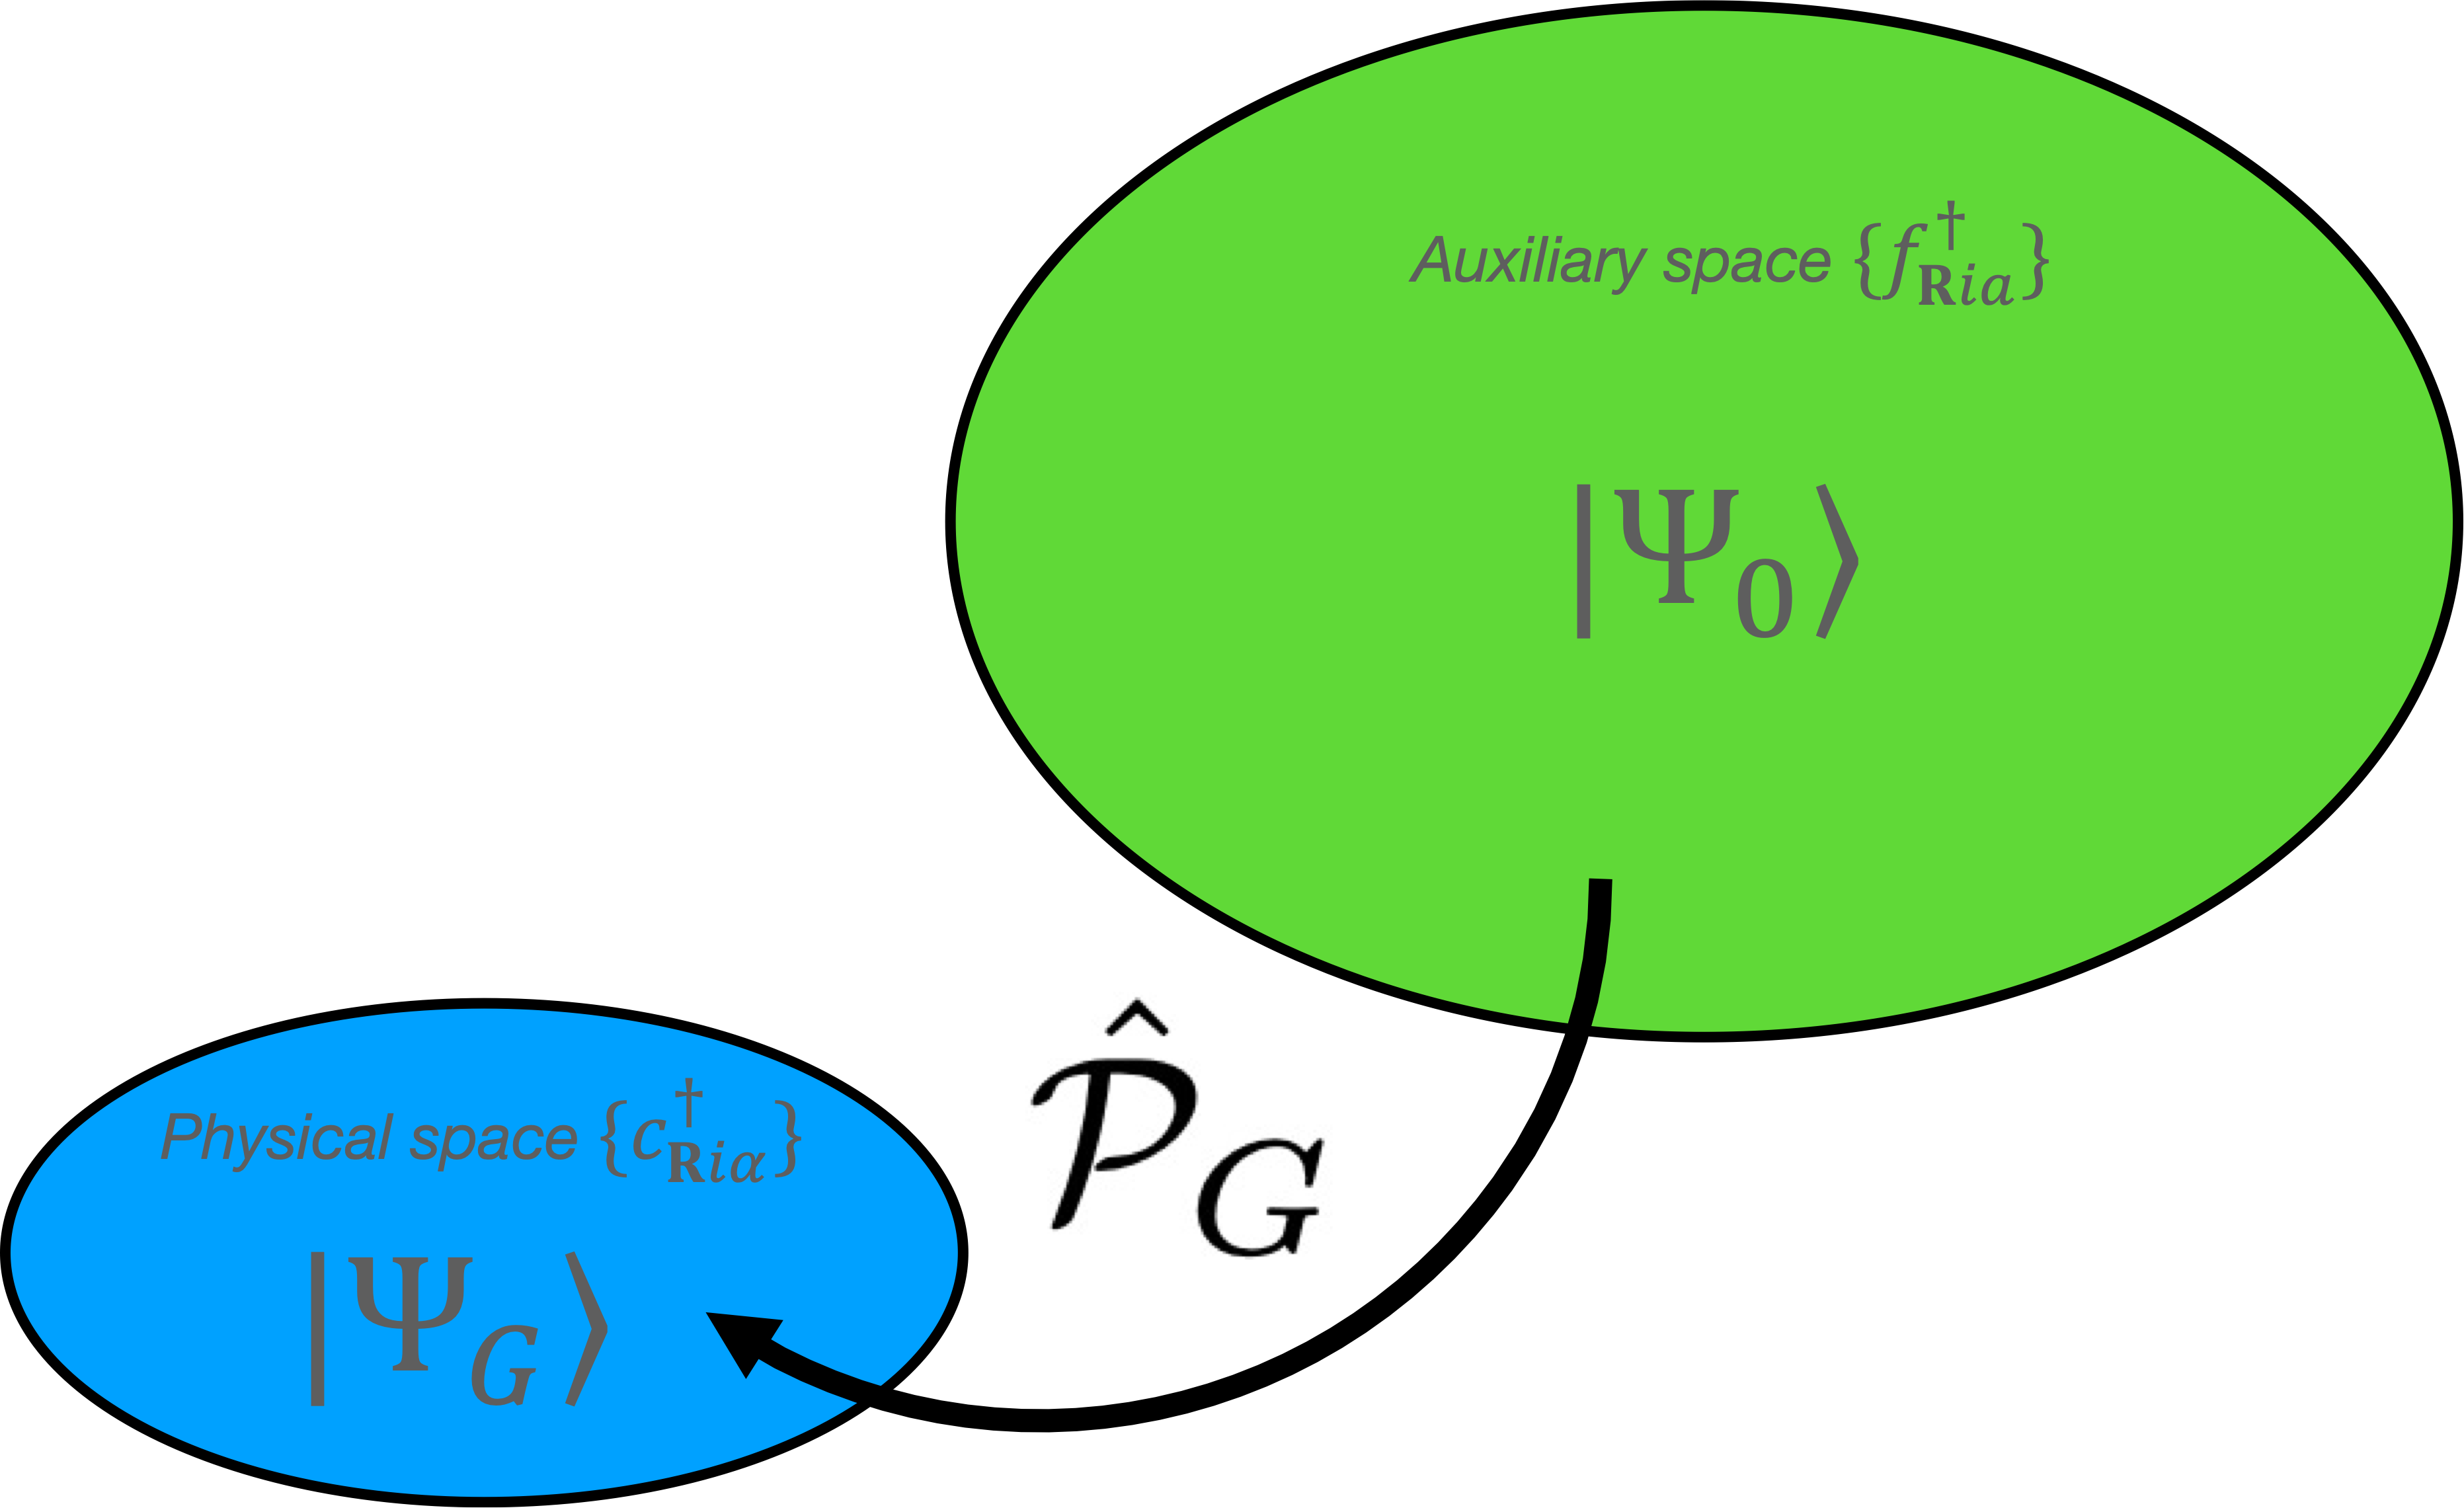
\includegraphics[width=7.7cm]{FigureS1}
    \caption{Schematic representation of the g-GA variational ansatz. The wavefunction $\ket{\Psi_G}$ is constructed by mapping a generic single-particle wavefunction $\ket{\Psi_0}$ constructed in an auxiliary Hilbert space, using the operator $\proj$.
    Both $\ket{\Psi_0}$ and $\proj$ are determined variationally}
    \label{FigureS1}
\end{figure}

\subsection{The $\text{g}$-GA variational ansatz}


The g-GA consists in minimizing the expectation value of $\h$
with respect to a wave function represented as follows:
\begin{align}
    \ket{\Psi_G}&=\proj\ket{\Psi_0}
\label{GWF}
\\
\proj&=\prod_{i\geq 1}\projRi
\,,
\end{align}
%
where $\ket{\Psi_0}$ is a single-particle wavefunction constructed in an auxiliary Hilbert space, generated by $\tilde{\nu}_i>\nu_i$ degrees of freedom $\fc_{\bR ia}$ $(a=1,..,\tilde{\nu}_i)$ for each $(\bR,i)$, while:
\begin{align}
\projRi&=\sum_{\Gamma=0}^{2^{\nu_i}-1}
\,
\sum_{n=0}^{2^{\tilde{\nu}_i}-1}
[\Lambda_{i}]_{\Gamma n}
\ket{\Gamma,{\bR i}}\bra{n,{\bR i}}
\\
\ket{\Gamma,{\bR i}}&=[\cc_{\bR i1}]^{q_1(\Gamma)} ...
[\cc_{\bR i q_{\nu_i}}]^{q_{\nu_i}(\Gamma)}\,\ket{0}
\\
\ket{n,{\bR i}}&=[\fc_{\bR i1}]^{q_1(n)} ...
[\fc_{\bR i q_{\tilde{\nu}_i}}]^{q_{\tilde{\nu}_i}(n)}\,\ket{0}
\end{align}
is an operator mapping the local auxiliary-space states into the physical space, see Fig.~\ref{FigureS1}, where $q_i(j)$ represents the $i$-th digit of $j$ in binary representation, and the matrix $\Lambda_i$ controls how $\projRi$
modifies the weight of the local electronic configurations.
%
The key reason why the g-GA variational ansatz generalizes the standard multi-orbital GA theory is that $\tilde{\nu}_i>\nu_i$.


In the present work we focus on the normal phase. Note that, to enforce the condition that $\ket{\Psi_G}$ is an eigenstate of the number operator, we do \emph{not}
need to assume that $\projRi$ commutes with the number operator, but only that:
\be
\sum_{j=1}^{\tilde{\nu}_i} q_j(n)-
\sum_{j=1}^{\nu_i} q_j(\Gamma)=m_i\quad
\forall\,\Gamma,n \, | \,
[\Lambda_i]_{\Gamma n}\neq 0\,,
\label{mi}
\ee
where $m_i$ is integer.
%
Our choice of $m_i$ (that, in principle, could be considered as an arbitrary variational parameter) will be specified below.



As in the standard multi-orbital GA, the variational wave function is restricted by the following
conditions:
\begin{align}
\Av{\Psi_0}{\projRidagger\projRi} &= \langle\Psi_0|\Psi_0\rangle=1
\label{gconstr1}
\\
\Av{\Psi_0}{\projRidagger\projRi\,\fc_{\bR ia}\fa_{\bR ib}} &=
\Av{\Psi_0}{\fc_{\bR ia}\fa_{\bR ib}}\qquad\forall\,a,b=1,...,\tilde{\nu}_i 
\,,
\label{gconstr2}
\end{align}
which are commonly called "Gutzwiller constraints".
%
Furthermore, the so-called "Gutzwiller Approximation", which becomes
exact in the limit of infinite coordination number~\cite{Gutzwiller3,GA-infinite-dim}
---where Dynamical Mean Field Theory (DMFT) is exact~\cite{DMFT}--- is assumed.


\subsection{The $\text{g}$-GA variational-energy components}

As in the standard multi-orbital GA, our goal is to evaluate the variational energy:
\be
\mathcal{E}(\Psi_0,\{\Lambda_i\})=\Av{\Psi_0}{\proj^\dagger\hat{H}\proj}\,.
\label{varen}
\ee
The only difference is that the operator $\proj^\dagger\hat{H}\proj$ and the operators appearing in Eqs.~\eqref{gconstr1}-\eqref{gconstr2}  reside within the auxiliary (extended) Hilbert space generated by the $\fc_{Ria}$ operators, where $a\in\{1,..,\tilde{\nu}_i\}$ and $\tilde{\nu}_i\geq \nu_i$.
%
In fact, if we set $\tilde{\nu}_i = \nu_i$ we recover exactly the original multi-orbital GA theory.



As we explain below for completeness, all of the formal steps leading to the quantum-embedding formulation of the GA can be essentially repeated for the g-GA following Ref.~\cite{Our-PRX}, even if $\tilde{\nu}_i > \nu_i$.
%
In particular, by employing the Gutzwiller approximation~\cite{Gutzwiller3,GA-infinite-dim}
and assuming the Gutzwiller constraints [Eqs.~\eqref{gconstr1},\eqref{gconstr2}], it can be shown that:
\begin{align}
\Av{\Psi_0}{\proj^\dagger\,\cc_{\bk i\alpha}\ca_{\bk j\beta}\,\proj}
&=\sum_{a=1}^{\tilde{\nu}_i}\sum_{b=1}^{\tilde{\nu}_j}
\Av{\Psi_0}{\left([\mathcal{R}_i]_{a\alpha}\fc_{\mathbf{R}ia}\right)\left([\mathcal{R}_j]^\dagger_{\beta b}\fa_{\mathbf{R}'jb}\right)}
\qquad\forall\,(\mathbf{R},i)\neq (\mathbf{R}',j)\,,
\label{hoppav}
\\
\Av{\Psi_0}{\proj^\dagger\,\h_{\bR i}^{\text{loc}}[\cc_{\bR i\alpha},\ca_{\bR i\alpha}]\,\proj}
&=\Av{\Psi_0}{\projRidagger\,\h_{\bR i}^{\text{loc}}[\cc_{\bR i\alpha},\ca_{\bR i\alpha}]\,\projRi}\,,
\label{locav}
\end{align}
where the $\tilde{\nu}_i\times \nu_i$ matrices $\mathcal{R}_i$ are the solution of the following linear equation:
\be
\Av{\Psi_0}{\projRidagger \cc_{\bR i\alpha}\projRi \fa_{\bR ia}}
=\sum_{b=1}^{\tilde{\nu}_i}[\mathcal{R}_i]_{b\alpha}
\Av{\Psi_0}{\fc_{\bR i b} \fa_{\bR ia}}\,.
\label{Rdef}
\ee


\subsection{Local $\ket{\Psi_0}$ averages as a function of variational parameters}

In the previous subsection we reduced the problem of evaluating the total-energy components to Eqs.~\eqref{hoppav}-\eqref{Rdef}.
%
Since all of these equations, as well as the Gutzwiller constraints [Eqs.~\eqref{gconstr1},\eqref{gconstr2}], involve expectation values with respect to $\ket{\Psi_0}$ of "local operators" (i.e., involving only $\fc_{\bR ia}$ and $\fa_{\bR ia}$ degrees of freedom at fixed $(\bR,i)$),
it is useful to introduce the corresponding local reduced density matrix of $\ket{\Psi_0}$.

By exploiting the fact that $\ket{\Psi_0}$ is a single-particle wavefunction (i.e., Wick's theorem applies to it), it can be readily verified that its reduced density matrix to the $(\bR,i)$ subsystem is given by:
\be
\hat{P}^0_{\bR i}\propto \exp\left\{-\sum_{a,b=1}^{\tilde{\nu}_i} \left[\ln\left(\frac{1-{^t\!\Delta_i}}{^t\!\Delta_i}\right)\right]_{ab}
\fc_{\bR i a} \fa_{\bR ib}
\right\}\,,
\label{hatp0}
\ee
where the entries of the $\tilde{\nu}_i\times \tilde{\nu}_i$ matrix $\Delta_i$ are given by:
\be
[\Delta_i]_{ab}=\Av{\Psi_0}{\fc_{\bR i a} \fa_{\bR ib}}
\ee
and ${^t\!\Delta_i}$ indicates the transpose of $\Delta_i$.

From the definitions above, it can be straightforwardly verified that:
\begin{align}
    \Av{\Psi_0}{\projRidagger\projRi}&=
    \Tr\big[P^0_i\Lambda^\dagger_i\Lambda^\dagga_i
    \big]
    \label{loc1}
    \\
    \Av{\Psi_0}{\projRidagger\projRi\,\fc_{\bR ia}\fa_{\bR ib}}&=
    \Tr\big[P^0_i\Lambda^\dagger_i\Lambda^\dagga_i
    \tilde{F}_{ia}^\dagger \tilde{F}_{ib}^\dagga
    \big]
    \\
    \Av{\Psi_0}{\projRidagger\,\h_{\bR i}^{\text{loc}}[\cc_{\bR i\alpha},\ca_{\bR i\alpha}]\,\projRi}&=
    \Tr\big[P^0_i\Lambda^\dagger_i
    \h_{\bR i}^{\text{loc}}[F^\dagger_{i\alpha},F^\dagga_{i\alpha}]
    \Lambda^\dagga_i\big]
    \\
    \Av{\Psi_0}{\projRidagger \cc_{\bR i\alpha}\projRi \fa_{\bR ia}}&=
    \Tr\big[P^0_i\Lambda^\dagger_i
    F_{i\alpha}^\dagger \Lambda^\dagga_i \tilde{F}_{ib}^\dagga\big]
    \label{loc4}
    \,,
\end{align}
where $\Tr$ is the trace and:
\begin{align}
    [{P}^0_{i}]_{nn'}&=\langle n,\mathbf{R}i |
    \hat{P}^0_{\bR i}
    | n', \mathbf{R}i\rangle
    \qquad (n,n'\in\{0,..,2^{\tilde{\nu}_i}-1\})
    \\
    [F_{i\alpha}]_{\Gamma\Gamma'}&=
    \langle \Gamma,\mathbf{R}i |
    \ca_{\bR i\alpha}
    | \Gamma', \mathbf{R}i\rangle
    \qquad (\Gamma,\Gamma'\in\{0,..,2^{{\nu}_i}-1\})
    \label{FGamma}
    \\
    [\tilde{F}_{ia}]_{nn'}&=
    \langle n,\mathbf{R}i |
    \fa_{\bR i a}
    | n', \mathbf{R}i\rangle
    \qquad (n,n'\in\{0,..,2^{\tilde{\nu}_i}-1\})
    \label{Fn}
    \,.
\end{align}




\subsection{Matrix of slave-boson amplitudes}

Following Refs.~\cite{lanata-barone-fabrizio,equivalence_GA-SB,Our-PRX}, 
we introduce the so-called matrix of slave-boson (SB)
amplitudes~\cite{Fresard1992,Georges,Lanata2016}:
\be
\phi_i=\Lambda_i\sqrt{P^0_i}\,.
\label{sba}
\ee

By substituting Eq.~\eqref{sba} in Eqs.~\eqref{loc1}-\eqref{loc4}, it can be readily verified that the Gutzwiller constraints can be rewritten as follows:
\begin{align}
\Tr\big[\phi^\dagger_i\phi^\dagga_i\big] &= \langle\Psi_0|\Psi_0\rangle=1
\label{gconstr1sb}
\\
\Tr\big[\phi^\dagger_i\phi^\dagga_i \tilde{F}_{ia}^\dagger \tilde{F}_{ib}^\dagga\big]
    &=
\Av{\Psi_0}{\fc_{\bR ia}\fa_{\bR ib}}=[\Delta_i]_{ab}
\qquad\forall\,a,b=1,...,\tilde{\nu}_i 
\label{gconstr2sb}
\end{align}
and that Eq.~\eqref{Rdef} can be rewritten as follows:
\be
\Tr\big[\phi^\dagger_i
    F_{i\alpha}^\dagger \phi^\dagga_i \tilde{F}_{ia}^\dagga\big]
=\sum_{c=1}^{\tilde{\nu}_i}[\mathcal{R}_i]_{c\alpha}\,
[\Delta_i(1-\Delta_i)]^{\frac{1}{2}}_{ca}
\,.
\label{Rdefsb}
\ee


\subsection{Embedding mapping}

Following Ref.~\cite{Our-PRX}, we introduce the so called "embedding states," which are related to the SB amplitudes as follows:
\begin{align}
    \ket{\Phi_i}=\sum_{\Gamma=0}^{2^{\nu_i}-1} \,\sum_{n=0}^{2^{\tilde{\nu}_i}-1}
    e^{i\frac{\pi}{2}N(n)(N(n)-1)}
    \,[\phi_i]_{\Gamma n} \,
    \ket{\Gamma;i}\otimes U_{\text{PH}}\ket{n;i}
    \label{ehstates}
\end{align}
where
\begin{align}
    \ket{\Gamma;i}&= [\hat{c}^\dagger_{i1}]^{q_1(\Gamma)} ...
[\hat{c}^\dagger_{i q_{\tilde{\nu}_i}}]^{q_{{\nu}_i}(\Gamma)}\,\ket{0}
    \\
    \ket{n;i}&= [\hat{f}^\dagger_{i1}]^{q_1(n)} ...
[\hat{f}^\dagger_{i q_{\tilde{\nu}_i}}]^{q_{\tilde{\nu}_i}(n)}\,\ket{0}
    \,,
\end{align}
$U_{\text{PH}}$ is a particle-hole transformation acting over the $\ket{n;i}$ states and
\be
N(n)=\sum_{a=1}^{\tilde{\nu}_i} q_a(n)
\,.
\ee

Note that the set of all embedding states represented as in Eq.~\eqref{ehstates} constitute a Fock space, corresponding to an "impurity" (generated by the Fermionic degrees of freedom $\hat{c}_{i\alpha}$, $\alpha\in\{1,..,\nu_i\}$) and a "bath" (generated by the Fermionic degrees of freedom $\hat{f}_{i a}$, $a\in\{1,..,\tilde{\nu}_i\}$).


The case $B=1$ corresponds to the standard GA theory, where the bath has the same size of the impurity.
%
In the present work we assumed that $\tilde{\nu}_i=B\nu_i$ and set $B=3$, see Fig.~\ref{FigureS2}.
%
Furthermore, we set $m_i=(\tilde{\nu}_i-\nu_i)/2=2$ (see Eq.~\eqref{mi}).
%
Note that, from the definitions [Eqs.~\eqref{sba},\eqref{ehstates}], it follows that this is equivalent to assume that 
$\ket{\Phi_i}$ has a total of $(\tilde{\nu}_i+\nu_i)/2=$4 electrons (i.e., that the embedding states are half-filled).
%




\begin{figure} %[htp]
    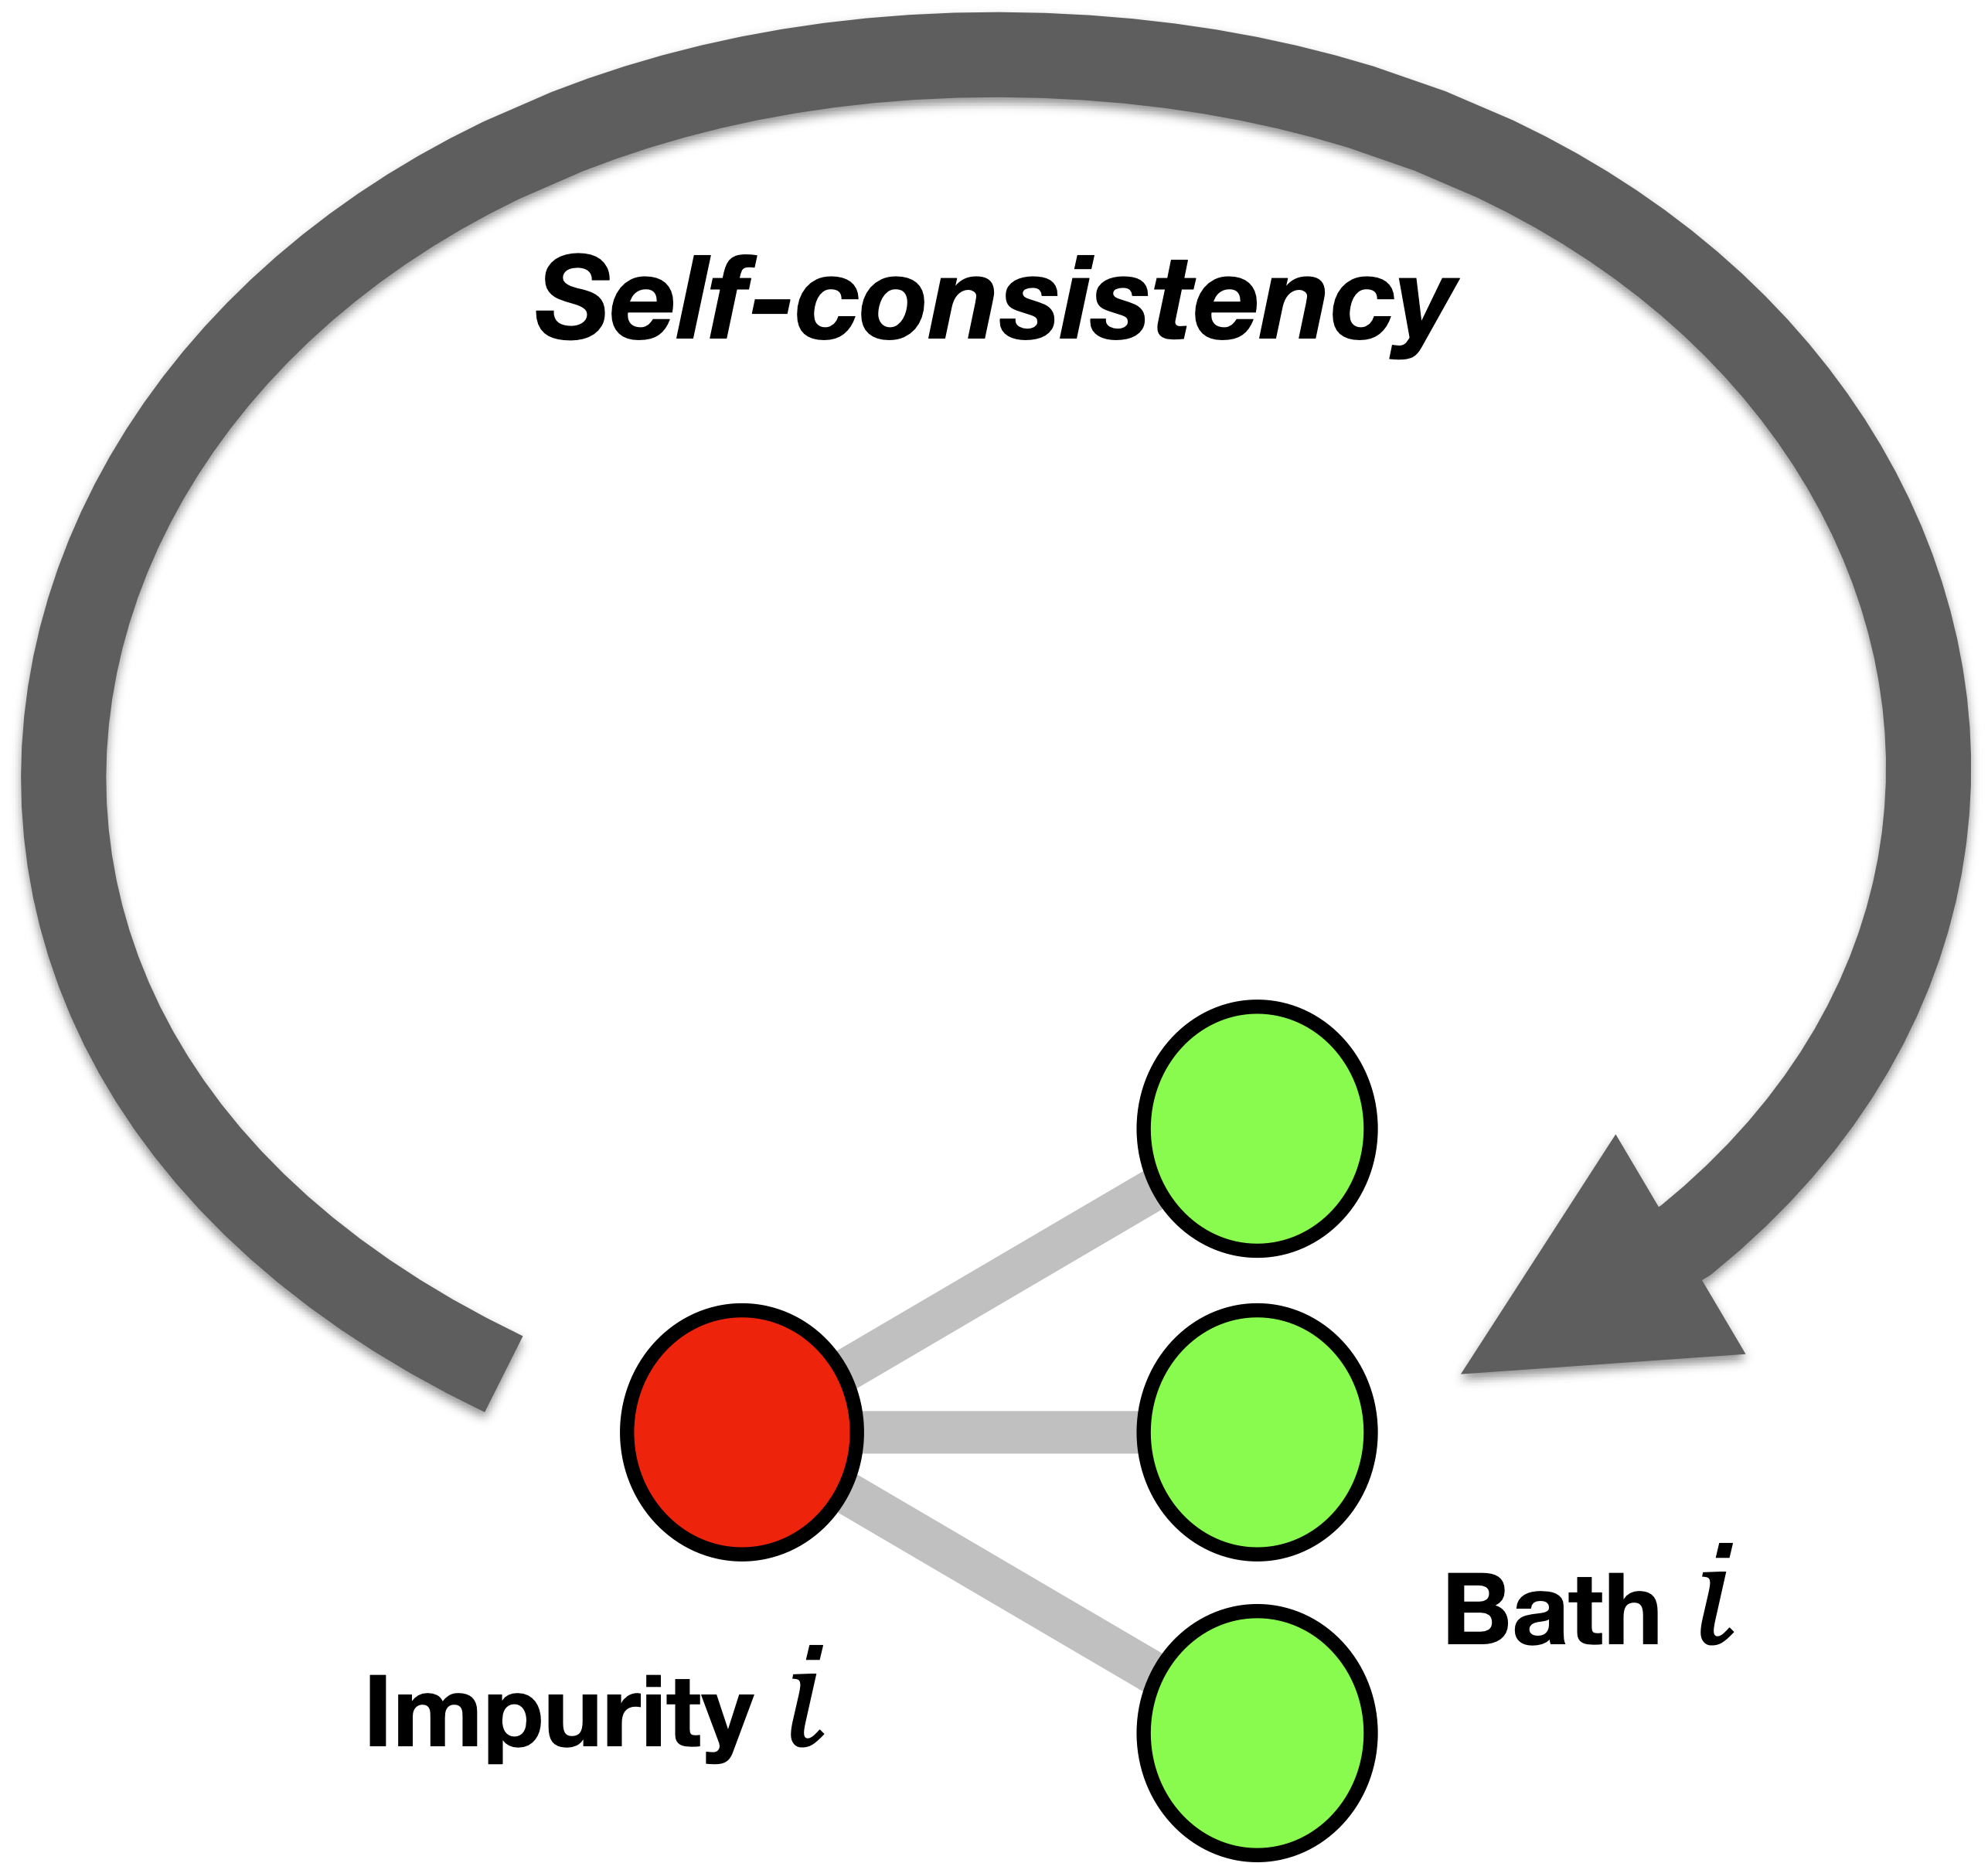
\includegraphics[width=7.7cm]{FigureS2}
    \caption{Schematic representation of the quantum-embedding algorithmic structure of the g-GA method. Here the number of bath sites $B=\tilde{\nu}_i/\nu_i$ (green circles) in the embedding Hamiltonian is set to $3$ (as in the calculations of the main text).
    }
    \label{FigureS2}
\end{figure}

It can be readily verified by inspection that the Gutzwiller constraints can be rewritten as follows:
\begin{align}
\langle\Phi_i|\Phi_i\rangle &= \langle\Psi_0|\Psi_0\rangle=1
\label{gconstr1eh}
\\
\Av{\Phi_i}{\hat{f}^\dagga_{i b}\hat{f}^\dagger_{i a}}
&=
\Av{\Psi_0}{\fc_{\bR ia}\fa_{\bR ib}}=[\Delta_i]_{ab}
\qquad\forall\,a,b=1,...,\tilde{\nu}_i 
,,
\label{gconstr2eh}
\end{align}
the expectation value of the local terms of $\hat{H}$ can be calculated as:
\be
\Av{\Psi_0}{\projRidagger\,\h_{\bR i}^{\text{loc}}[\cc_{\bR i\alpha},\ca_{\bR i\alpha}]\,\projRi} =
\Av{\Phi_i}{\h_{\bR i}^{\text{loc}}[\hat{c}^\dagger_{ i\alpha},\hat{c}^\dagga_{i\alpha}]}
\ee
and that Eq.~\eqref{Rdef} can be rewritten as:
\be
\Av{\Psi_0}{\hat{c}^\dagger_{i \alpha}\hat{f}^\dagger_{i a}}
=\sum_{c=1}^{\tilde{\nu}_i}[\mathcal{R}_i]_{c\alpha}\,
[\Delta_i(1-\Delta_i)]^{\frac{1}{2}}_{ca}
\,.
\label{Rdefeh}
\ee

In summary, by substituting Eqs.~\eqref{hoppav} and \eqref{locav} in Eq.~\eqref{varen}
and using the equations above,
we deduce that the goal is to minimize the following expression for the variational energy:
\be
\mathcal{E}=
\sum_{\bR\bR'}\sum_{i,j\geq 0}\sum_{a,b=1}^{\bar{\nu}_i}\left[\R_i^\dagga t_{\bR i,\bR'j}\R^{\dagger}_j\right]_{ab} \fc_{\bR ia}\fa_{\bR' jb}
+
\sum_{\bR}\sum_{i\geq 1}
\Av{\Phi_i}{\h_{\bR i}^{\text{loc}}[\hat{c}^\dagger_{ i\alpha},\hat{c}^\dagga_{i\alpha}]}
\ee
while fulfilling the Gutzwiller constraints [Eqs.~\eqref{gconstr1eh}, \eqref{gconstr2eh}].






\subsection{Lagrange formulation of the g-GA} \label{covariance-sec}

Following Refs.~\onlinecite{Our-PRX,Lanata2016,Ghost-GA}, the constrained energy-minimization problem described above can be cast in terms of the following Lagrange function:

\bea
&&\Lag[
{\Phi},E^c;\,  \R,\lambda;\, \D, \lambda^{c};\,\Delta, \Psi_0, E]=
%
\frac{1}{\mathcal{N}}\Av{\Psi_0}{\h_{\text{qp}}[\R,\lambda]}
+E\!\left(1\!-\!\langle\Psi_0|\Psi_0\rangle\right)
\nonumber\\&&\quad\quad
+\sum_{i\geq 1}\left[\Av{\Phi_i}{\h_i^{\text{emb}}[\D_i,\lambda_i^c]}
+E^c_i\!\left(1-\langle \Phi_i | \Phi_i \rangle
\right)\right]
\nonumber\\&&\quad\quad
-\sum_{i\ge 1}\left[
\sum_{a,b=1}^{\tilde{\nu}_i}\big(
\left[\lambda_i\right]_{ab}+\left[\lambda^c_i\right]_{ab}\big)\left[\Delta_{i}\right]_{ab}
+\sum_{c,a=1}^{\tilde{\nu}_i}\sum_{\alpha=1}^{\nu_i}
\big(
\left[\D_{i}\right]_{a\alpha}\left[\R_{i}\right]_{c\alpha}
\left[\Delta_{i}(1-\Delta_{i})\right]^{\frac{1}{2}}_{ca}
+\text{c.c.}\big)
\right]\,,
\label{Lag-SB-emb}
\eea
%
where $\mathcal{N}$ is the total number of unit cells,
$E$ and $E^c$ are real numbers, $\Delta_i$, $\lambda^c_i$ and $\lambda_i$ are
$\tilde{\nu}_i\times \tilde{\nu}_i$ Hermitian matrices, $\D_i$ and $\R_i$ are generic (rectangular) $\tilde{\nu}_i\times {\nu}_i$ matrices.
%
%
The auxiliary Hamiltonians $\Hqp$ and $\h_{\text{emb}}$,
which are called "quasiparticle Hamiltonian" and "Embedding Hamiltonian,"
respectively, are defined as follows:
\begin{align}
    \h_{\text{qp}}&=\sum_{\bR\bR'}\sum_{i,j\geq 0}\sum_{a,b=1}^{\bar{\nu}_i}\left[\R_i^\dagga t_{\bR i,\bR'j}\R^{\dagger}_j\right]_{ab}
    \fc_{\bR ia}\fa_{\bR' jb}
    + \sum_{\bR}\sum_{i\geq 0}\sum_{a,b=1}^{\bar{\nu}_i} \left[ \lambda_i \right]_{ab}\fc_{\bR ia} \fa_{\bR ib}
    \label{hqp}
    \\
    \h_i^{\text{emb}}&= \hat{H}^{\mathrm{loc}}_{i}\big[\{\hat{c}^{\dagger}_{ i},\hat{c}^{\phantom{\dagger}}_{i}\} \big] + \sum_{a=1}^{\tilde{\nu}_i}\sum_{\alpha=1}^{\nu_i}\left[\D_i\right]_{a\alpha}\hat{c}^{\dagger}_{i\alpha}\hat{f}^{\phantom{\dagger}}_{ia}
   +\sum_{a,b=1}^{\tilde{\nu}_i}\left[\lambda^c_i\right]_{ab}\hat{f}^{\phantom{\dagger}}_{ib}\hat{f}^{\dagger}_{ia}
   \quad\forall\,i\geq 1
   \,.
   \label{hemb}
\end{align}

The saddle-point of the Lagrangian $\Lag$ defined in Eq. \eqref{Lag-SB-emb} is given by the following equations:
\begin{align}
    &\frac{1}{\mathcal{N}} \left[\sum_{\bk}\Pi_if\left(\R t_{\bk}\R^{\dagger}+\lambda\right)\Pi_i\right]_{ba} = \left[\Delta_i\right]_{ab}
    \label{detDelta}
    \\
    &\frac{1}{\mathcal{N}}\left[\sum_{\bk}\Pi_i 
    t_{\bk}\R^{\dagger} f\left(\R t_{\bk}\R^{\dagger}+\lambda\right)\Pi_i\right]_{\alpha a} = \sum_{c,a=1}^{\tilde{\nu}_i}\sum_{\alpha=1}^{\nu_i}\left[\D_i\right]_{c\alpha}\left[\Delta_i\left(1-\Delta_i\right)\right]^{\tfrac{1}{2}}
    \label{detD}
    \\
   &\sum_{c,b=1}^{\tilde{\nu}_i}\sum_{\alpha=1}^{\nu_i}\frac{\partial}{\partial \left[d^0_i\right]_s} \left(\left[\Delta_i\left(1-\Delta_i\right)\right]^{\tfrac{1}{2}}_{cb}\left[\D_i\right]_{b\alpha}\left[\R_i\right]_{c\alpha} + \mathrm{c.c.}\right) + [l_i+l^c_i]_{s} = 0
   \label{detLc}
   \\
   &\h_i^{\mathrm{emb}}\ket{\Phi_i} = E_i^c\ket{\Phi_i}
   \\
   &\left[\F_i^{(1)}\right]_{\alpha a} = \bra{\Phi_i}\hat{c}^{\dagger}_{i\alpha}\hat{f}^{\phantom{\dagger}}_{ia}\ket{\Phi_i}
   - \sum_{c=1}\left[\Delta_i\left(1-\Delta_i\right)\right]^{\tfrac{1}{2}}\left[\R_i\right]_{c\alpha} \overset{!}{=} 0
   \label{detF1}
   \\
   &\left[\F_i^{(2)}\right]_{ab} = \bra{\Phi_i}\hat{f}^{\phantom{\dagger}}_{ib}\hat{f}^{\dagger}_{ia}\ket{\Phi_i} - \left[\Delta_i\right]_{ab} \overset{!}{=} 0
   \,,
   \label{detF2}
\end{align}
where $f$ is the zero-temperature Fermi function and in Eqs.~\eqref{detDelta},\eqref{detD} we introduced the following block-matrices:
\begin{align}
   \label{blockL}
   \lambda = \begin{pmatrix}
    \left[\mathbf{0}\right]_{\nu_0\times\nu_0} & \dots & \dots & \mathbf{0} \\
    \vdots & \lambda_1 &  \vdots \\
    \vdots & \vdots &  \ddots & \vdots \\
    \mathbf{0} & \dots &  \dots & \lambda_M
  \end{pmatrix} 
  \,,
\end{align}

\begin{align}
   \label{blockR}
   \R = \begin{pmatrix}
    \left[\mathbf{1}\right]_{\nu_0\times\nu_0}  &\dots& \dots & \mathbf{0} \\
    \mathbf{0} & \R_1 & \dots & \vdots \\
    \vdots  & \vdots  & \ddots & \vdots \\
    \mathbf{0} & \dots& \dots & \R_M
  \end{pmatrix}
  \,,
\end{align}
where $\left[\mathbf{1}\right]_{n\times n}$ is the $n\times n$ identity matrix
and $\left[\mathbf{0}\right]_{n\times n}$ is the $n\times n$ zero matrix.
%
We also introduced the following projectors:
\begin{align}
   \label{Proj}
   \Pi_i = \begin{pmatrix}
    \delta_{i0}\left[\mathbf{1}\right]_{\nu_0\times\nu_0} & \dots &\dots & \mathbf{0} \\
    \vdots & \delta_{i1}\left[\mathbf{1}\right]_{\tilde{\nu}_1\times\tilde{\nu}_1} & \dots & \vdots \\
    \vdots & \vdots  & \ddots & \vdots \\
    \mathbf{0}  & \dots& \dots & \delta_{iM}\left[\mathbf{1}\right]_{\tilde{\nu}_M\times\tilde{\nu}_M}
  \end{pmatrix}
  \,.
\end{align}
%
Finally, we introduced the following expansions of the matrices $\Delta_i$, $\lambda_i$, $\lambda^c_i$, in terms of an orthonormal
basis of Hermitian matrices $\left\{\left[h_i\right]_s\right\}$ (with respect to the canonical scalar product $(A, B) = \Tr \left[A^{\dagger}B\right]$):
\begin{align}
    \label{coeffDelta}
    \Delta_i =& \sum_{s=1}^{\tilde{\nu}_i^2} \left[d^0_i\right]_s {}^t\left[h_i\right]_s \\
    \label{coeffL}
    \lambda_i =& \sum_{s=1}^{\tilde{\nu}_i^2} \left[l_i\right]_s \left[h_i\right]_s  \\
    \label{coeffLc}
    \lambda^c_i =& \sum_{s=1}^{\tilde{\nu}_i^2} \left[l^c_i\right]_s \left[h_i\right]_s \,,
\end{align}
where $\left[d^0_i\right]_s$, $\left[l_i\right]_s$ and $\left[l^c_i\right]_s$ are real-valued coefficients.




\subsection{Algorithmic structure of the g-GA}
The equations \eqref{detDelta}-\eqref{detF2} can be solved numerically using the following numerical procedure (represented schematically in Fig.~\ref{FigureS2}):
\begin{enumerate}
    \item Starting from an initial guess for the coefficients $\left[r_i\right]_a$ and $\left[l_i\right]_s$ construct the matrix $\R_i$ directly by using $\left[r_i\right]_a$ as the matrix elements of $\R_i$ and the matrix $\lambda_i$ according to Eq. \eqref{coeffL}.
    \item Arrange the $\R_i$ and $\lambda_i$ in block matrices over all $i$ as shown in Eqs. \eqref{blockL} and \eqref{blockR} and construct $\h_{\mathrm{qp}}$ as shown in Eq.\eqref{hqp}.
    \item Compute $\Delta_i$ according to Eq. \eqref{detDelta} using the projector $\Pi_i$ as given in Eq. \eqref{Proj}.
    \item Compute the Lagrange multipliers $\D_i$ by inverting Eq. \eqref{detD}.
    \item Determine the coefficients $\left[l^c_i\right]_s$ from Eq. \eqref{detLc} and construct the matrix $\lambda^c_i$ according to Eq. \eqref{coeffLc}.
    \item Construct $\h^{\mathrm{emb}}_i$ according to Eq.~\eqref{hemb} and calculate its ground state $\ket{\Phi_i}$ within the subspace with $(\nu_i+\tilde{\nu}_i)/2$ electrons (i.e., half of the total number of EH modes).
    \item Compute $\F_i^{(1)}$ and $\F_i^{(2)}$ according to equations \eqref{detF1} and \eqref{detF2}.
\end{enumerate}
A saddle-point of $\Lag$ satisfies $\F_i^{(1)}=\F_i^{(2)}=0$, i.e.,
the procedure described above has to be repeated until a self-consistent solution to these equations is found.




\subsection{Gauge invariance of the g-GA} \label{sec:Gauge}

Following Ref. \onlinecite{Lanata2016} it can be readily shown that also the g-GA Lagrangian is invariant with respect to the following Gauge transformation:
\begin{align}
    \ket{\Psi_0} &\rightarrow \U^{\dagger}\left(\theta\right)\ket{\Psi_0} 
    \label{g1}
    \\
    \ket{\Phi_i} &\rightarrow U_i^{\dagger}\left(\theta_i\right)\ket{\Phi_i} \\
    \R_i &\rightarrow u^{\dagger}_i\left(\theta_i\right)\R_i \\
    \D_i &\rightarrow {}^t u\left(\theta_i\right)\D_i \\
    \Delta_i &\rightarrow {}^t u_i\left(\theta_i\right)\Delta_i {}^t u_i^{\dagger}\left(\theta_i\right) \\
    \lambda_i &\rightarrow u_i^{\dagger}\left(\theta_i\right)\lambda_i u_i \left(\theta_i\right) \\
    \lambda_i^c &\rightarrow u_i^{\dagger}\left(\theta_i\right) \lambda_i^c u_i\left(\theta_i\right)
    \label{g7}
    \,,
\end{align}
with:
\begin{align}
    u_i\left(\theta_i\right) &= e^{i\theta_i} \\
    U_i\left(\theta_i\right) &= e^{i\sum_{a,b=1}^{\tilde{\nu}_i}\left[\theta_i\right]_{ab} \hat{f}^{\dagger}_{ia}\hat{f}^{\phantom{\dagger}}_{ib}} \\
    \U\left(\theta\right) &= e^{i\sum_{R}\sum_{i\geq 1}\sum_{a,b=1}^{\tilde{\nu}_i}\left[\theta_i\right]_{ab} \fc_{Ria}\fa_{Rib}} \,,
\end{align}
where $u_i\left(\theta_i\right)\in\mathbb{C}^{\tilde{\nu}_i\times\tilde{\nu}_i}$, $U_i\left(\theta_i\right)\in\mathbb{C}^{2^{\tilde{\nu}_i}\times 2^{\tilde{\nu}_i}}$
and $\U\left(\theta\right)\in\mathbb{C}^{2^{\tilde{\nu}}\times 2^{\tilde{\nu}}}$ and $\theta_i$ are Hermitian matrices.






\subsection{General analytical expression for spectral function from g-GA variational parameters}

Let us consider the g-GA zero-temperature spectral function, defined as follows:
\be
\mathcal{A}_{i\alpha,j\beta}(\bk,\omega)=
\Av{\Psi_G}{\ca_{\bk i \alpha}\,\delta(\omega-\h)\,\cc_{\bk j \beta}}+
\Av{\Psi_G}{\cc_{\bk j \beta}\,\delta(\omega+\h)\,\ca_{\bk i \alpha}}\,.
\label{Ghost-Ak}
\ee
%
Following Ref.~\onlinecite{Ghost-GA}, we obtain the
following approximation to the physical Green's function:
\be
\mathcal{G}_{i\alpha,j\beta}(\bk,\omega)=\int_{-\infty}^{\infty}d\epsilon\,
\frac{\mathcal{A}_{i\alpha,j\beta}(\bk,\omega)}{\omega-\epsilon}
\simeq\left[
\R^\dagger_i\,\Pi_i\frac{1}{\omega-[\R \epsilon_{\bk}
	\R^\dagger+\lambda]}\Pi_j\,\R_j
\right]_{\alpha\beta}
\,.
\label{tG}
\ee



As explained above, 
the g-GA Lagrange function is invariant under the group of gauge transformations defined by Eqs.~\eqref{g1}-\eqref{g7}.
%
To calculate the self-energy, it is convenient to
choose a gauge such that $\lambda_i$ is diagonal and decompose $R_i$ and $\lambda_i$ as follows:
\begin{align}
    \R_i &= \begin{pmatrix} \R_i^{(1)} \\ \R_i^{(2)} \end{pmatrix} 
    \label{decR}
    \\
    \lambda_i &= \begin{pmatrix} \lambda_i^{(1)} & \mathbf{0} \\ \mathbf{0} & \lambda_i^{(2)} \end{pmatrix}
    \,,
    \label{lambdadec}
\end{align}
where $\R_i^{(1)}$ and $\lambda_i^{(1)}$ are matrices of dimension $\nu_i\times\nu_i$, while $\R_i^{(2)}$ and $\lambda_i^{(2)}$ are $(\tilde{\nu}_i-\nu_i)\times\nu_i$ and 
$(\tilde{\nu}_i-\nu_i)\times(\tilde{\nu}_i-\nu_i)$, respectively.
%
In this gauge, using Eqs.~\eqref{decR}, \eqref{lambdadec} and the Dyson equation:
\begin{align}
    \G(\bk,\omega) = \left[\omega - \tau_{\bk}-\Sigma(\omega)\right]^{-1}
\end{align}
(where $\tau_{\bk} = t_{\bk} + t^{\mathrm{loc}}$
also contains all local terms of Eq.~\eqref{hloc-quadratic}),
%
it can be shown with a straightforward calculation that the self-energy is given by the following equation:
\begin{align}
   \Sigma(\omega) = \begin{pmatrix}
    \left[\mathbf{0}\right]_{\nu_0\times\nu_0} &\mathbf{0}& \dots & \mathbf{0} \\
    \mathbf{0} & \Sigma_1(\omega) & \dots &\vdots \\
    \vdots & \vdots  & \ddots & \vdots \\
    \mathbf{0} & \dots& \dots & \Sigma_M(\omega)
  \end{pmatrix}
  \,,
\end{align}
where, as expected, $\Sigma(\omega)$ is local ($\bk$-independent) and
$\Sigma_i(\omega)$ are the $\nu_i\times\nu_i$ matrices $\forall\,i\geq 1$, given by the following equation:
\begin{align}
    \Sigma_{i}(\omega) =& t^{\mathrm{loc}}_i -\omega\frac{\mathbf{1}-\R_i^{(1)\dagger}\R_i^{(1)}}{\R_i^{(1)\dagger}\R_i^{(1)}} +\left[\R_i^{(1)}\right]^{-1} \lambda^{(1)}_i\left[\R_i^{(1)\dagger}\right]^{-1} + \left[\R_i^{(1)}\right]^{-1}\left(\omega-\lambda_i^{(1)}\right)\left[\R_i^{(1)\dagger}\right]^{-1}\R_i^{(2)\dagger} \nonumber\\ 
    &\times
    \Biggl[\R_i^{(2)}\left[\R_i^{(1)}\right]^{-1}\left(\omega-\lambda^{(1)}_i\right)\left[\R_i^{(1)\dagger}\right]^{-1}\R_i^{(2)\dagger}+\left(\omega-\lambda_i^{(2)}\right)\Biggr]^{-1}
    \nonumber\\
    &\times\R_i^{(2)}\left[\R_i^{(1)}\right]^{-1} \left(\omega-\lambda_i^{(1)}\right)\left[\R_i^{(1)\dagger}\right]^{-1}
    \,,
\end{align}
which reduces to Eq.~10 of the main text for single-orbital impurities.

Note that, as pointed out in the main text, from Eq.~\eqref{tG} it follows that the poles of the Green's function lie on top of the eigenvalues of the quasi-particle Hamiltonian, see Eq.~\eqref{hqp}.
%
However, because of the matrices $\mathcal{R}^\dagger_i$ and $\mathcal{R}_j$ at the left and the right of Eq.~\eqref{tG} ---which are rectangular, ---
only a portion of the quasi-particle spectral weight is physical (see Fig.~3 of the main text).



\section{Pathology of the bare GA in the narrow-bandwidth limit of the ALM}


\begin{figure} %[htp]
    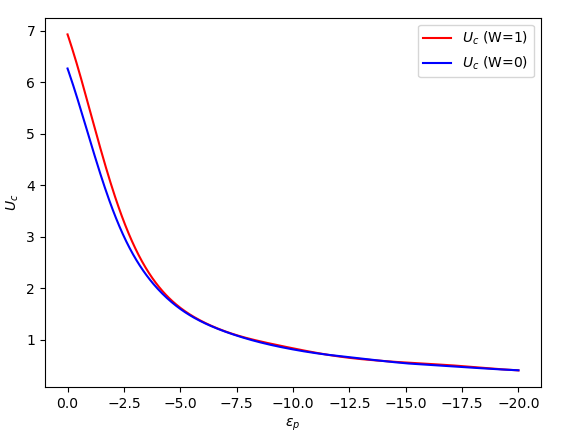
\includegraphics[width=11.7cm]{FigureS3}
    \caption{Behavior of $U_c$ as a function of $\epsilon_p$ in bare GA for $V=1$, both for $W=1$ (red) and in the narrow-bandwidth limit $W=0$ (blue).
    }
    \label{FigureS3}
\end{figure}

As pointed out in the main text, within the GA the Mott transition of the ALM occurs (by construction) only when
$\langle\dc_{i\sigma}\pa_{i\sigma}
    \rangle_{\text{GA}}
    =r 
    \Av{\Psi_0}{\fc_{i\sigma}\pa_{i\sigma}}=0$,
i.e., when the variational parameter $r$ vanishes.
%
However, as shown in Fig.~1 of the main text, the GA critical value $U_c$ is overestimated dramatically for the ALM, especially for $\epsilon_p\ll -1$.


To explain this behavior, it is insightful to inspect the GA solution also in the narrow-bandwidth limit, i.e., setting the half-bandwidth $W$ of the Bethe-lattice hopping matrix to $0$ ---corresponding to a series of decoupled $p$-$d$ dimers.
%
The resulting evolution of $U_c$ (i.e., the interaction strength such that $r$ vanishes) is shown here in Fig.~\ref{FigureS3}, where we set
$V=1$ and consider $\epsilon_p\ll -1$.


We observe that, not surprisingly (since $V=1$),
$\langle\dc_{i\sigma}\pa_{i\sigma} \rangle_{\text{GA}}$ does not vanish at $U\sim 0$ (neither for $W=0$ nor for $W=1$).
In fact, at $U=0$ the $GA$ wavefunction is exact.
%
On the other hand, in this limit any infinitesimal $U$ should induce a Mott transition for $W\rightarrow 0$.
%
This simple observation showcases very clearly how, as pointed out in the main text, the $p$-$d$ charge fluctuations cannot be neglected in the Mott phase ---as they \emph{must} coexist in the narrow-bandwidth limit of the ALM.
%
In other words, the argument above shows that ---for small $W$--- the GA behavior of $U_c$ is essentially unrelated with the Mott transition.
%%
We also note that, for the values of $\epsilon_p$ considered in Fig.~\ref{FigureS3}, the GA behavior of $U_c$ is almost independent of whether $W=0$ or $W=1$.
%
In fact, one can readily demonstrate also analytically that the bare GA predicts that $U_c(W)\sim U_c(W=0)\sim V^{2}/\left|\epsilon_{p}\right|$ $\forall\,W$ for $\epsilon_p\rightarrow -\infty$ (which is clearly incorrect).
%(see the analytical proof in the subsection below).
%
This shows that the pathology of the GA, that we discussed above in the narrow-bandwidth limit, cannot be only regarded as an accident specific to this particular  case,
as it affects the GA predictions also for finite $W$.

In summary, while the bare GA captures some qualitative features of the phase diagram of the ALM, here we identified a pathological behavior of this method in the narrow-bandwidth limit, which leads to a dramatic overestimation of $U_c$ (especially for $\epsilon_p\rightarrow -\infty$).
%
From a general perspective, this problem can be traced back to the inability of the GA of describing simultaneously the Mott physics and the $p$-$d$ charge fluctuations.
%
In the main text we showed that the g-GA does not have such limitation and, consequently, it resolves the problems of the bare GA here uncovered, providing us with a description of the ALM with accuracy comparable to DMFT.


%\subsection{Behavior of $U_c$ for $\epsilon_p\ll -1$}

%In this limit, we expect  the two-band problem to be reduced to a single-band Hubbard model. This effective model has a bandwidth that, at leading order of $1/\left|\epsilon_{p}\right|$, is $W_{eff}\sim W\times V^{2}/\left|\epsilon_{p}\right|^{2}$, with the pre-factor depending on the lattice considered. The physical expectation is that a Mott transition occurs when the interaction $U_{c}$ is of order of $W_{eff}$. This is not, however, what happens at the GA approach. Simple algebra~\cite{Kotliar-Ruckenstein} leads to a critical value of $U_{c}\sim V^{2}/\left|\epsilon_{p}\right|$, independent of $W$. This result implies that a transition is predicted by the GA even when $W$ is zero, clearly a limitation of the technique. In general, $U_{c}\sim W_{eff}\times\left|\epsilon_{p}\right|/W$, showing, generically, a huge overestimation of $U_{c}$ when $\left|\epsilon_{p}\right|\gg W$. 


%%\bibliography{ref}

%apsrev4-2.bst 2019-01-14 (MD) hand-edited version of apsrev4-1.bst
%Control: key (0)
%Control: author (8) initials jnrlst
%Control: editor formatted (1) identically to author
%Control: production of article title (0) allowed
%Control: page (0) single
%Control: year (1) truncated
%Control: production of eprint (0) enabled
\begin{thebibliography}{15}%
\makeatletter
\providecommand \@ifxundefined [1]{%
 \@ifx{#1\undefined}
}%
\providecommand \@ifnum [1]{%
 \ifnum #1\expandafter \@firstoftwo
 \else \expandafter \@secondoftwo
 \fi
}%
\providecommand \@ifx [1]{%
 \ifx #1\expandafter \@firstoftwo
 \else \expandafter \@secondoftwo
 \fi
}%
\providecommand \natexlab [1]{#1}%
\providecommand \enquote  [1]{``#1''}%
\providecommand \bibnamefont  [1]{#1}%
\providecommand \bibfnamefont [1]{#1}%
\providecommand \citenamefont [1]{#1}%
\providecommand \href@noop [0]{\@secondoftwo}%
\providecommand \href [0]{\begingroup \@sanitize@url \@href}%
\providecommand \@href[1]{\@@startlink{#1}\@@href}%
\providecommand \@@href[1]{\endgroup#1\@@endlink}%
\providecommand \@sanitize@url [0]{\catcode `\\12\catcode `\$12\catcode
  `\&12\catcode `\#12\catcode `\^12\catcode `\_12\catcode `\%12\relax}%
\providecommand \@@startlink[1]{}%
\providecommand \@@endlink[0]{}%
\providecommand \url  [0]{\begingroup\@sanitize@url \@url }%
\providecommand \@url [1]{\endgroup\@href {#1}{\urlprefix }}%
\providecommand \urlprefix  [0]{URL }%
\providecommand \Eprint [0]{\href }%
\providecommand \doibase [0]{https://doi.org/}%
\providecommand \selectlanguage [0]{\@gobble}%
\providecommand \bibinfo  [0]{\@secondoftwo}%
\providecommand \bibfield  [0]{\@secondoftwo}%
\providecommand \translation [1]{[#1]}%
\providecommand \BibitemOpen [0]{}%
\providecommand \bibitemStop [0]{}%
\providecommand \bibitemNoStop [0]{.\EOS\space}%
\providecommand \EOS [0]{\spacefactor3000\relax}%
\providecommand \BibitemShut  [1]{\csname bibitem#1\endcsname}%
\let\auto@bib@innerbib\@empty
%</preamble>
\bibitem [{\citenamefont {Lanat\`a}\ \emph {et~al.}(2017)\citenamefont
  {Lanat\`a}, \citenamefont {Lee}, \citenamefont {Yao},\ and\ \citenamefont
  {Dobrosavljevi\ifmmode~\acute{c}\else \'{c}\fi{}}}]{Ghost-GA}%
  \BibitemOpen
  \bibfield  {author} {\bibinfo {author} {\bibfnamefont {N.}~\bibnamefont
  {Lanat\`a}}, \bibinfo {author} {\bibfnamefont {T.-H.}\ \bibnamefont {Lee}},
  \bibinfo {author} {\bibfnamefont {Y.-X.}\ \bibnamefont {Yao}},\ and\ \bibinfo
  {author} {\bibfnamefont {V.}~\bibnamefont
  {Dobrosavljevi\ifmmode~\acute{c}\else \'{c}\fi{}}},\ }\bibfield  {title}
  {\bibinfo {title} {Emergent $\text{B}$loch excitations in $\text{M}$ott
  matter},\ }\href@noop {} {\bibfield  {journal} {\bibinfo  {journal} {Phys.
  Rev. B}\ }\textbf {\bibinfo {volume} {96}},\ \bibinfo {pages} {195126}
  (\bibinfo {year} {2017})}\BibitemShut {NoStop}%
\bibitem [{\citenamefont {Anisimov}\ \emph
  {et~al.}(1997{\natexlab{a}})\citenamefont {Anisimov}, \citenamefont
  {Oteryaev}, \citenamefont {Korotin}, \citenamefont {Anokhin},\ and\
  \citenamefont {Kotliar}}]{Anisimov_DMFT}%
  \BibitemOpen
  \bibfield  {author} {\bibinfo {author} {\bibfnamefont {V.~I.}\ \bibnamefont
  {Anisimov}}, \bibinfo {author} {\bibfnamefont {A.~I.}\ \bibnamefont
  {Oteryaev}}, \bibinfo {author} {\bibfnamefont {M.~A.}\ \bibnamefont
  {Korotin}}, \bibinfo {author} {\bibfnamefont {A.~O.}\ \bibnamefont
  {Anokhin}},\ and\ \bibinfo {author} {\bibfnamefont {G.}~\bibnamefont
  {Kotliar}},\ }\bibfield  {title} {\bibinfo {title} {First-principles
  calculations of the electronic structure and spectra of strongly correlated
  systems: dynamical mean-field theory},\ }\href@noop {} {\bibfield  {journal}
  {\bibinfo  {journal} {J. Phys. Condens. Matter}\ }\textbf {\bibinfo {volume}
  {9}},\ \bibinfo {pages} {7359} (\bibinfo {year}
  {1997}{\natexlab{a}})}\BibitemShut {NoStop}%
\bibitem [{\citenamefont {Deng}\ \emph {et~al.}(2009)\citenamefont {Deng},
  \citenamefont {Wang}, \citenamefont {Dai},\ and\ \citenamefont
  {Fang}}]{Fang}%
  \BibitemOpen
  \bibfield  {author} {\bibinfo {author} {\bibfnamefont {X.-Y.}\ \bibnamefont
  {Deng}}, \bibinfo {author} {\bibfnamefont {L.}~\bibnamefont {Wang}}, \bibinfo
  {author} {\bibfnamefont {X.}~\bibnamefont {Dai}},\ and\ \bibinfo {author}
  {\bibfnamefont {Z.}~\bibnamefont {Fang}},\ }\bibfield  {title} {\bibinfo
  {title} {Local density approximation combined with {Gutzwiller} method for
  correlated electron systems: {Formalism} and applications},\ }\href@noop {}
  {\bibfield  {journal} {\bibinfo  {journal} {Phys. Rev. B}\ }\textbf {\bibinfo
  {volume} {79}},\ \bibinfo {eid} {075114} (\bibinfo {year}
  {2009})}\BibitemShut {NoStop}%
\bibitem [{\citenamefont {Lanat\`a}\ \emph {et~al.}(2015)\citenamefont
  {Lanat\`a}, \citenamefont {Yao}, \citenamefont {Wang}, \citenamefont {Ho},\
  and\ \citenamefont {Kotliar}}]{Our-PRX}%
  \BibitemOpen
  \bibfield  {author} {\bibinfo {author} {\bibfnamefont {N.}~\bibnamefont
  {Lanat\`a}}, \bibinfo {author} {\bibfnamefont {Y.-X.}\ \bibnamefont {Yao}},
  \bibinfo {author} {\bibfnamefont {C.-Z.}\ \bibnamefont {Wang}}, \bibinfo
  {author} {\bibfnamefont {K.-M.}\ \bibnamefont {Ho}},\ and\ \bibinfo {author}
  {\bibfnamefont {G.}~\bibnamefont {Kotliar}},\ }\bibfield  {title} {\bibinfo
  {title} {Phase diagram and electronic structure of praseodymium and
  plutonium},\ }\href@noop {} {\bibfield  {journal} {\bibinfo  {journal} {Phys.
  Rev. X}\ }\textbf {\bibinfo {volume} {5}},\ \bibinfo {pages} {011008}
  (\bibinfo {year} {2015})}\BibitemShut {NoStop}%
\bibitem [{\citenamefont {Anisimov}\ \emph
  {et~al.}(1997{\natexlab{b}})\citenamefont {Anisimov}, \citenamefont
  {Aryasetiawan},\ and\ \citenamefont {Lichtenstein}}]{LDA+U}%
  \BibitemOpen
  \bibfield  {author} {\bibinfo {author} {\bibfnamefont {V.~I.}\ \bibnamefont
  {Anisimov}}, \bibinfo {author} {\bibfnamefont {F.}~\bibnamefont
  {Aryasetiawan}},\ and\ \bibinfo {author} {\bibfnamefont {A.~I.}\ \bibnamefont
  {Lichtenstein}},\ }\bibfield  {title} {\bibinfo {title} {First-principles
  calculations of the electronic structure and spectra of strongly correlated
  systems: the $\text{LDA+U}$ method},\ }\href@noop {} {\bibfield  {journal}
  {\bibinfo  {journal} {J. Phys. Condens. Matter}\ }\textbf {\bibinfo {volume}
  {9}},\ \bibinfo {pages} {767} (\bibinfo {year}
  {1997}{\natexlab{b}})}\BibitemShut {NoStop}%
\bibitem [{\citenamefont {Haule}\ \emph {et~al.}(2010)\citenamefont {Haule},
  \citenamefont {Yee},\ and\ \citenamefont {Kim}}]{Haule10}%
  \BibitemOpen
  \bibfield  {author} {\bibinfo {author} {\bibfnamefont {K.}~\bibnamefont
  {Haule}}, \bibinfo {author} {\bibfnamefont {C.-H.}\ \bibnamefont {Yee}},\
  and\ \bibinfo {author} {\bibfnamefont {K.}~\bibnamefont {Kim}},\ }\bibfield
  {title} {\bibinfo {title} {Dynamical mean-field theory within the
  full-potential methods: Electronic structure of $\text{CeIrIn}_{5}$,
  $\text{CeCoIn}_{5}$, and $\text{CeRhIn}_{5}$},\ }\href
  {https://doi.org/10.1103/PhysRevB.81.195107} {\bibfield  {journal} {\bibinfo
  {journal} {Phys. Rev. B}\ }\textbf {\bibinfo {volume} {81}},\ \bibinfo
  {pages} {195107} (\bibinfo {year} {2010})}\BibitemShut {NoStop}%
\bibitem [{\citenamefont {Lechermann}\ \emph {et~al.}(2006)\citenamefont
  {Lechermann}, \citenamefont {Georges}, \citenamefont {Poteryaev},
  \citenamefont {Biermann}, \citenamefont {Posternak}, \citenamefont
  {Yamasaki},\ and\ \citenamefont {Andersen}}]{PWF2}%
  \BibitemOpen
  \bibfield  {author} {\bibinfo {author} {\bibfnamefont {F.}~\bibnamefont
  {Lechermann}}, \bibinfo {author} {\bibfnamefont {A.}~\bibnamefont {Georges}},
  \bibinfo {author} {\bibfnamefont {A.}~\bibnamefont {Poteryaev}}, \bibinfo
  {author} {\bibfnamefont {S.}~\bibnamefont {Biermann}}, \bibinfo {author}
  {\bibfnamefont {M.}~\bibnamefont {Posternak}}, \bibinfo {author}
  {\bibfnamefont {A.}~\bibnamefont {Yamasaki}},\ and\ \bibinfo {author}
  {\bibfnamefont {O.~K.}\ \bibnamefont {Andersen}},\ }\bibfield  {title}
  {\bibinfo {title} {Dynamical mean-field theory using $\text{Wannier}$
  functions: $\text{A}$ flexible route to electronic structure calculations of
  strongly correlated materials},\ }\href
  {https://doi.org/10.1103/PhysRevB.74.125120} {\bibfield  {journal} {\bibinfo
  {journal} {Phys. Rev. B}\ }\textbf {\bibinfo {volume} {74}},\ \bibinfo
  {pages} {125120} (\bibinfo {year} {2006})}\BibitemShut {NoStop}%
\bibitem [{\citenamefont {Gutzwiller}(1965)}]{Gutzwiller3}%
  \BibitemOpen
  \bibfield  {author} {\bibinfo {author} {\bibfnamefont {M.~C.}\ \bibnamefont
  {Gutzwiller}},\ }\bibfield  {title} {\bibinfo {title} {Correlation of
  {Electrons} in a {Narrow} {$s$} {Band}},\ }\href
  {https://doi.org/10.1103/PhysRev.137.A1726} {\bibfield  {journal} {\bibinfo
  {journal} {Phys. Rev.}\ }\textbf {\bibinfo {volume} {137}},\ \bibinfo {pages}
  {A1726} (\bibinfo {year} {1965})}\BibitemShut {NoStop}%
\bibitem [{\citenamefont {Metzner}\ and\ \citenamefont
  {Vollhardt}(1989)}]{GA-infinite-dim}%
  \BibitemOpen
  \bibfield  {author} {\bibinfo {author} {\bibfnamefont {W.}~\bibnamefont
  {Metzner}}\ and\ \bibinfo {author} {\bibfnamefont {D.}~\bibnamefont
  {Vollhardt}},\ }\bibfield  {title} {\bibinfo {title} {Correlated lattice
  fermions in $d=\ensuremath{\infty}$ dimensions},\ }\href@noop {} {\bibfield
  {journal} {\bibinfo  {journal} {Phys. Rev. Lett.}\ }\textbf {\bibinfo
  {volume} {62}},\ \bibinfo {pages} {324} (\bibinfo {year} {1989})}\BibitemShut
  {NoStop}%
\bibitem [{\citenamefont {Georges}\ \emph {et~al.}(1996)\citenamefont
  {Georges}, \citenamefont {Kotliar}, \citenamefont {Krauth},\ and\
  \citenamefont {Rozenberg}}]{DMFT}%
  \BibitemOpen
  \bibfield  {author} {\bibinfo {author} {\bibfnamefont {A.}~\bibnamefont
  {Georges}}, \bibinfo {author} {\bibfnamefont {G.}~\bibnamefont {Kotliar}},
  \bibinfo {author} {\bibfnamefont {W.}~\bibnamefont {Krauth}},\ and\ \bibinfo
  {author} {\bibfnamefont {M.~J.}\ \bibnamefont {Rozenberg}},\ }\bibfield
  {title} {\bibinfo {title} {Dynamical mean-field theory of strongly correlated
  fermion systems and the limit of infinite dimensions},\ }\href@noop {}
  {\bibfield  {journal} {\bibinfo  {journal} {Rev. Mod. Phys.}\ }\textbf
  {\bibinfo {volume} {68}},\ \bibinfo {pages} {13} (\bibinfo {year}
  {1996})}\BibitemShut {NoStop}%
\bibitem [{\citenamefont {Lanat\`{a}}\ \emph {et~al.}(2008)\citenamefont
  {Lanat\`{a}}, \citenamefont {Barone},\ and\ \citenamefont
  {Fabrizio}}]{lanata-barone-fabrizio}%
  \BibitemOpen
  \bibfield  {author} {\bibinfo {author} {\bibfnamefont {N.}~\bibnamefont
  {Lanat\`{a}}}, \bibinfo {author} {\bibfnamefont {P.}~\bibnamefont {Barone}},\
  and\ \bibinfo {author} {\bibfnamefont {M.}~\bibnamefont {Fabrizio}},\
  }\bibfield  {title} {\bibinfo {title} {Fermi-surface evolution across the
  magnetic phase transition in the {Kondo} lattice model},\ }\href@noop {}
  {\bibfield  {journal} {\bibinfo  {journal} {Phys. Rev. B}\ }\textbf {\bibinfo
  {volume} {78}},\ \bibinfo {eid} {155127} (\bibinfo {year}
  {2008})}\BibitemShut {NoStop}%
\bibitem [{\citenamefont {B\"unemann}\ and\ \citenamefont
  {Gebhard}(2007)}]{equivalence_GA-SB}%
  \BibitemOpen
  \bibfield  {author} {\bibinfo {author} {\bibfnamefont {J.}~\bibnamefont
  {B\"unemann}}\ and\ \bibinfo {author} {\bibfnamefont {F.}~\bibnamefont
  {Gebhard}},\ }\bibfield  {title} {\bibinfo {title} {Equivalence of
  $\text{Gutzwiller}$ and slave-boson mean-field theories for multiband
  $\text{Hubbard}$ models},\ }\href@noop {} {\bibfield  {journal} {\bibinfo
  {journal} {Phys. Rev. B}\ }\textbf {\bibinfo {volume} {76}},\ \bibinfo
  {pages} {193104} (\bibinfo {year} {2007})}\BibitemShut {NoStop}%
\bibitem [{\citenamefont {Fr{\'{e}}sard}\ and\ \citenamefont
  {W{\"{o}}lfle}(1992)}]{Fresard1992}%
  \BibitemOpen
  \bibfield  {author} {\bibinfo {author} {\bibfnamefont {R.}~\bibnamefont
  {Fr{\'{e}}sard}}\ and\ \bibinfo {author} {\bibfnamefont {P.}~\bibnamefont
  {W{\"{o}}lfle}},\ }\bibfield  {title} {\bibinfo {title} {Unified slave boson
  representation of spin and charge degrees of freedom for strongly correlated
  fermi systems},\ }\href {https://doi.org/10.1142/S0217979292000414}
  {\bibfield  {journal} {\bibinfo  {journal} {International Journal of Modern
  Physics B}\ }\textbf {\bibinfo {volume} {06}},\ \bibinfo {pages} {685}
  (\bibinfo {year} {1992})}\BibitemShut {NoStop}%
\bibitem [{\citenamefont {Lechermann}\ \emph {et~al.}(2007)\citenamefont
  {Lechermann}, \citenamefont {Georges}, \citenamefont {Kotliar},\ and\
  \citenamefont {Parcollet}}]{Georges}%
  \BibitemOpen
  \bibfield  {author} {\bibinfo {author} {\bibfnamefont {F.}~\bibnamefont
  {Lechermann}}, \bibinfo {author} {\bibfnamefont {A.}~\bibnamefont {Georges}},
  \bibinfo {author} {\bibfnamefont {G.}~\bibnamefont {Kotliar}},\ and\ \bibinfo
  {author} {\bibfnamefont {O.}~\bibnamefont {Parcollet}},\ }\bibfield  {title}
  {\bibinfo {title} {Rotationally invariant slave-boson formalism and momentum
  dependence of the quasiparticle weight},\ }\href@noop {} {\bibfield
  {journal} {\bibinfo  {journal} {Phys. Rev. B}\ }\textbf {\bibinfo {volume}
  {76}},\ \bibinfo {eid} {155102} (\bibinfo {year} {2007})}\BibitemShut
  {NoStop}%
\bibitem [{\citenamefont {Lanat{\`{a}}}\ \emph {et~al.}(2017)\citenamefont
  {Lanat{\`{a}}}, \citenamefont {Yao}, \citenamefont {Deng}, \citenamefont
  {Dobrosavljevi{\'{c}}},\ and\ \citenamefont {Kotliar}}]{Lanata2016}%
  \BibitemOpen
  \bibfield  {author} {\bibinfo {author} {\bibfnamefont {N.}~\bibnamefont
  {Lanat{\`{a}}}}, \bibinfo {author} {\bibfnamefont {Y.-X.}\ \bibnamefont
  {Yao}}, \bibinfo {author} {\bibfnamefont {X.}~\bibnamefont {Deng}}, \bibinfo
  {author} {\bibfnamefont {V.}~\bibnamefont {Dobrosavljevi{\'{c}}}},\ and\
  \bibinfo {author} {\bibfnamefont {G.}~\bibnamefont {Kotliar}},\ }\bibfield
  {title} {\bibinfo {title} {{Slave Boson Theory of Orbital Differentiation
  with Crystal Field Effects: Application to UO$_2$}},\ }\href@noop {}
  {\bibfield  {journal} {\bibinfo  {journal} {Phys. Rev. Lett.}\ }\textbf
  {\bibinfo {volume} {118}},\ \bibinfo {pages} {126401} (\bibinfo {year}
  {2017})}\BibitemShut {NoStop}%
\end{thebibliography}%




\end{document}


 
